
Este experimento es muy parecido al anterior. El circuito auxiliar a utilizar será el mismo (con algunas modificaciones en sus conexiones), pero en este caso la impedancia a medir será la impedancia de entrada $Z_i$. 

Se comenzó de la misma manera que en el experimento anterior, desconectando el jumper $J2$ y midiendo la máxima tensión de salida en vacío sin que recorte. Como se esperaba, este valor fue el mismo que en el caso anterior, $v_s$ = 10,2 $V_{pp}$.

Una vez hecho esto, se configuró el circuito de la siguiente manera (figura \ref{fig:circ2}):

\begin{figure}[H]
    \centering
    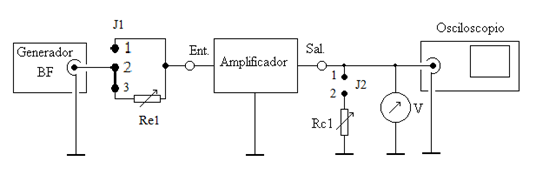
\includegraphics[width=0.9\textwidth]{Imagenes/conexZiLA.png}
    \caption{Conexión del Amplificador de prueba para medir la impedancia de entrada}
    \label{fig:circ2}
\end{figure}

La conexión de $J1$ entre 2 y 3, sitúa entre la salida del generador y la entrada del amplificador, una resistencia variable $R_{e_1}$, que servirá para determinar el valor de $Z_i$. 

En este punto, muy similarmente a la experiencia anterior, se varió el valor de $R_{e_1}$, hasta obtener en la salida del amplificador una señal con una amplitud igual a la mitad de la amplitud obtenida en vacío. Luego se desconecto el generador y la fuente del circuito, se retiró el jumper $J1$ y se midió el valor de $R_{e_1}$. Igual que antes, este debería ser una representación bastante acertada del valor de impedancia de entrada del amplificador. 

\subsubsection{Mediciones}

Los datos obtenidos en estas mediciones están expuestos en la tabla \ref{tab:exp2}.

Nuevamente las mediciones fueron realizadas con el multímetro de la marca UNI-T, modelo UT890C.

%poner tabla exp2 una vez lista y bien hecha la de la exp1

\begin{table}[H]
    \centering
    \scalebox{1}{
    \begin{tabular} {|c|c|c|c|c|}
    %{|m{1.5cm}|m{2.7cm}|m{1cm}|p{1.5cm}|m{2.7cm}|}
   
    \hline
         $f$ & Valor Nominal & $V_s$ & $R_{e_1}=R_i$ & Incertidumbre \\
         
         Frec. Gen. & de $Z_{ent}=R_i$ & en vacío & Para $V_s'=\frac{V_s}{2}$ & medición $R_{e_1}$\\
    \hline
        1 kHz & 1 k$\ohm$ & 10.2 $V_{pp}$ & 1102 $\Omega$ & $\pm$ 8.819 $\Omega$ \\
    \hline
        \end{tabular}}
        \def\tablename{Tabla} 
        \caption{Valores esperados y obtenidos}
        \label{tab:exp2}
\end{table}

Se puede observar que el valor de impedancia de entrada obtenido a partir de la resistencia medida, es muy similar al valor nominal (esperado), por lo que se lo puede considerar un valor realista y que la medición dio lo que se esperaba. 

En este caso el valor resultó ser un poco más grande de lo esperado, lo que en el caso de los amplificadores es una característica positiva, ya que, el amplificador ideal se espera que tenga una impedancia de entrada infinita.